%% Advances in Combinatorics article template
%%
%% aic-template.tex v0.33
%%
%% AUTHOR: Fill in fields (or see warnings) below marked with "AUTHOR"
%% ** Add as few macro / package definitions as possible
%% ** Compile with "pdflatex"; make sure that
%%           aic.cls and tocbase.cls are in the same directory.
%%
%% EDITOR: Fill in fields below marked with "EDITOR"
%%    and check that authors properly filled in field marked with "AUTHOR"

\documentclass{aic}

\usepackage[utf8]{inputenc}
\usepackage{tikz}
\usetikzlibrary{fit}
\usepackage{bbm}
\usepackage[shortlabels]{enumitem}
\usepackage{thmtools}
\usepackage{mathtools}

\newcommand{\pcb}{polynomially $\chi$-bounded}
\newcommand{\qpcb}{quasi-polynomially $\chi$-bounded}

\declaretheorem[name=Lemma, numberwithin = section]{lemma}
\declaretheorem[name=Theorem,sibling = lemma]{theorem}
\declaretheorem[name=Proposition, sibling=lemma]{proposition}
\declaretheorem[name=Definition, sibling=lemma]{definition}
\declaretheorem[name=Corollary, sibling=lemma]{corollary}
\declaretheorem[name=Conjecture, sibling=lemma]{conjecture}
\declaretheorem[name=Problem, sibling=lemma]{problem}
\declaretheorem[name=Remark, sibling=lemma]{remark}
\declaretheorem[name=Claim]{claim}

%%%%%%%%%%%%%%%%%%%%%%%%%%%%%%%%%%%%%%%%%%%%%%%%
%% AUTHOR: Fill in meta-data below:
\aicAUTHORdetails{%
  title = {Bounded Twin-Width Graphs are Polynomially $\chi$-Bounded}, %% please capitalize all significant words
  author = {Romain Bourneuf and Stéphan Thomassé},
    %% Please use the format for commas as follows:
    %% "A", or "A and B", or "A, B, and C", or "A, B, C, and D", etc.
  plaintextauthor = {Romain Bourneuf, Stéphan Thomassé},
    %% An author list in plain text: Use the format
    %% "A", or "A, B", or "A, B, C", etc.
    %% NOTE: No LaTeX code in author names.
    %% NOTE: No "and" at the end--simply comma separated,
    % 
 %% The remaining lines in this section are optional:
    %
%     %% IF YOUR TITLE CONTAINS MATH OR LATEX such as accented characters: 
%     %% Add a "plain text title";  otherwise comment out the next line:
%   plaintexttitle = {Short Proof of Rodl's n**loglog n Bound}, %%  title without math or LaTeX
%     %
%     %% ONLY IF YOUR TITLE IS TOO LONG to fit in the page headers, please 
%     %% add an abbreviated version of the title, otherwise comment it out:
%   runningtitle = {R\"odl's $n^{\log\log n}$ Bound}, 
%     %
%     %% ONLY IF YOUR AUTHOR LIST IS TOO LONG to fit in the page headers, 
%     %% add an abbreviated version, otherwise comment it out:
%   runningauthor = {Paul Erd\H{o}s, Johan H{\aa}stad, L\'aszl\'o Lov\'asz, and Andrew C-C. Yao},
%     %% you can replace first names and/or middle names with initials.
%     %
%     %% ONLY IF YOUR AUTHOR LIST IS TOO LONG to fit the copyright entry
%     %% on the bottom of the front page,
%     %% add an abbreviated version, otherwise comment it out:
%   copyrightauthor = {P. Erd\H{o}s, J. H{\aa}stad, L. Lov\'asz, and A. C-C. Yao},
%     %% Note that the copyrightauthor  field will seldom be necessary;
%     %% for instance, in this example with four authors, it would be 
%     %% all right to comment it out and have all authors' full names 
%     %% appear on the Copyright line
%    %
%    %% Include keywords of your choice: comma separated, lower case;
%    %% comment out the "keywords" line if you don't wish to provide them
%   keywords = {keyword, keyword, etc.},
 }   %%% END \aicAUTHORdetails

%%%%%%%%%%%%%%%%%%%%%%%%%%%%%%%%%%%%%%%%%%%%%%%%
%%% EDITOR: please fill in the following data:
\aicEDITORdetails{%
   year={2025},
   %volume={XX},
   number={2},
   received={28 March 2023},   % received date: example: 7 January 2017
 %  revised={XX Month 20XX},    % Optional revised date (you may comment it out)
   published={13 February 2025},  % published date
   doi={10.19086/aic.2025.2},      % XXX = number of paper, e.g. aic006 for paper#6
%                              % or  aic0006 (length of string arbitrary)
}   %%% END \aicEDITORdetails

\begin{document}

\begin{frontmatter}[classification=text]
%% EDITOR: this will force the keywords to appear right after the Abstract.
%%   If the abstract is too long and would force the keywords off the
%%   front page, please comment out % [classification=text] above
%%   This way the keywords will be floated on the bottom of the first page
%%   even though the Abstract spills over to the next page.

%%% AUTHOR: Title goes here.  This line is optional.  You must use it
%%   if title has footnote attached or requires nontrivial typesetting,
%%   e.g., inclusion of linebreaks to force nice layout.
%\title{Bounded Twin-Width Graphs are Polynomially $\chi$-Bounded} %% please capitalize all significant words

%%% AUTHOR:
%%% List all authors. If you wish, place grant acknowledgements in \thanks.
%%% In brackets include a short tag for each author.
\author[rom]{Romain Bourneuf}
\author[stef]{Stéphan Thomassé\thanks{This work was supported by ANR Digraphs
ANR-19-CE48-0013
}}

%%% AUTHOR: Abstract goes here
\begin{abstract}
We show that every graph with twin-width $t$ has chromatic number $O(\omega ^{k_t})$ for some integer $k_t$, where $\omega$ denotes the clique number. This extends a quasi-polynomial bound from Pilipczuk and Soko\l{}owski and generalizes a result for bounded clique-width graphs by Bonamy and Pilipczuk. The proof uses the main ideas of the quasi-polynomial approach, with a different treatment of the decomposition tree. In particular, we identify two types of extensions of a class of graphs: the delayed-extension (which preserves polynomial $\chi$-boundedness) and the right-extension (which preserves polynomial $\chi$-boundedness under bounded twin-width condition). Our main result is that every bounded twin-width graph is a delayed extension of simpler classes of graphs, each expressed as a bounded union of right extensions of lower twin-width graphs.
\end{abstract}
\end{frontmatter}

%%% AUTHOR: body of paper starts here

\section{Introduction}
\label{sec:introduction}
% \begin{itemize}
%     % Diffusion of FL
%     \item {\st{Diffusion of FL}}
%     % Security threats to FL
%     \item {\st{Security threats to FL with particular focus on model poisoning}}
%     % Limitations of existing countermeasures
%     \item {\st{Current countermeasures (e.g., KRUM) and their limitations}}
%     % Proposed method and its advantages
%     \item {\st{Intuitive description of the proposed method and its difference (i.e., advantages) w.r.t. state of the art}}
%     % Main contributions
%     \item {\st{Summary of the main contributions of this work}}
%     % Paper's structure and organization
%     \item {\st{Paper's structure and organization}}
% \end{itemize}

% Diffusion of FL
Recently, {\em federated learning} (FL) has emerged as the leading paradigm for training distributed, large-scale, and privacy-preserving machine learning (ML) systems~\cite{mcmahan2017googleai,mcmahan2017aistats}. 
The core idea of FL is to allow multiple edge clients to collaboratively train a shared, global model without disclosing their local private training data.
%Specifically, an FL system consists of a central server and many edge clients; 
A typical FL round involves the following steps: {\em(i)} the server randomly picks some clients and sends them the current, global model; {\em(ii)} each selected client locally trains its model with its own private data; then, it sends the resulting local model to the server;\footnote{Whenever we refer to global/local model, we mean global/local model {\em parameters}.} {\em(iii)} the server updates the global model by computing an \emph{aggregation function}, usually the average (FedAvg), on the local models received from clients.
% \begin{enumerate}
%     \item[{\em(i)}] the server sends the current, global model to the clients and appoints some of them for training;
%     \item[{\em(ii)}] each selected client locally trains its copy of the global model with its own private data; then, it sends the resulting local model back to the server;\footnote{Whenever we refer to global/local model, we mean global/local model {\em parameters}.}
%     \item[{\em(iii)}] the server updates the global model by computing an \emph{aggregation function} on the local models received from clients (by default, the average, also referred to as FedAvg~\cite{mcmahan2017aistats}).
% \end{enumerate}
This process goes on until the global model converges. %(e.g., after a certain number of rounds or other similar stopping criteria).
%\\
% The advantages of FL over the traditional, centralized learning paradigm are undoubtedly clear in terms of flexibility/scalability (clients can join/disconnect from the FL network dynamically), network communications (only model weights\footnote{We will use \textit{parameters} and \textit{weights} interchangeably.} are exchanged between clients and server), and privacy (each client's private training data is kept local at the client's end and not uploaded to the server).
\\
% Security threats to FL
%However, the growing adoption of FL also raises security concerns~\cite{costa2022covert}, particularly about its confidentiality, integrity, and availability.
Although its advantages over standard ML, FL also raises security concerns~\cite{costa2022covert}. %, particularly about its confidentiality, integrity, and availability~\cite{costa2022covert}.
% OLD, LONG VERSION
% Indeed, some work deals with privacy leakage that may expose the local data of some clients~\cite{melis2019sp}. 
% A large body of work, instead, investigates attacks that usually aim to detriment the predictive accuracy of the learned global model. For instance, \emph{data poisoning} attacks achieve this goal by letting an adversary pollute the training set of some corrupt FL clients with maliciously crafted examples~\cite{jagielski2018sp}.
% Similarly, in \emph{model poisoning} the attacker attempts to tweak the global model weights~\cite{bhagoji2019pmlr} by directly perturbing the local model's weights of some infected FL clients before these are sent to the central server for aggregation, usually via so-called Byzantine attacks. 
% It turns out that Byzantine model poisoning attacks severely impact standard FedAvg; therefore, more robust aggregation functions must be designed to make FL systems secure.
Here, we focus on \emph{untargeted model poisoning} attacks~\cite{bhagoji2019pmlr}, where an adversary attempts to tweak the global model weights %\footnote{We will use the terms \textit{parameters} and \textit{weights} interchangeably.} 
by directly perturbing the local model's parameters of some infected clients before these are sent to the central server for aggregation.
In doing so, the adversary aims to jeopardize the global model \textit{indiscriminately} at inference time.
Such model poisoning attacks severely impact standard FedAvg; therefore, more robust aggregation functions must be designed to secure FL systems.
\\
% In this paper, we focus on designing a novel robust aggregation scheme at the server's end to contrast the effect of Byzantine model poisoning attacks.
%
% Current countermeasures and their limitations
%Several countermeasures have been proposed in the literature to combat model poisoning attacks on FL systems.
% Some methods use simple statistics more robust than plain average to smooth the impact of malicious updates (e.g., Trimmed Mean and FedMedian~\cite{yin2018icml}). 
% Other defenses implement outlier detection techniques to discard malicious updates from the aggregation performed at the server's end. Those are either based on heuristics (e.g., Krum/Multi-Krum~\cite{blanchard2017nips} and Bulyan~\cite{mhamdi2018pmlr}) or data-driven approaches (e.g., K-means clustering~\cite{shen2016acm} or DnC via spectral analysis~\cite{shejwalkar2021ndss}). 
% Finally, some strategies rely on a centralized ``source of trust'' to spot potential malicious updates (e.g., FLTrust~\cite{cao2020fltrust}).
% Several countermeasures have been proposed in the literature to combat model poisoning attacks on FL systems, i.e., to discard possible malicious local updates from the aggregation performed at the server's end. 
% These techniques range from simple statistics more robust than plain average (e.g., Trimmed Mean and FedMedian~\cite{yin2018icml}) to outlier detection heuristics (e.g., Krum/Multi-Krum~\cite{blanchard2017nips} and Bulyan~\cite{mhamdi2018pmlr}) or data-driven approaches (e.g., spectral analysis via K-means clustering~\cite{shen2016acm} or spectral analysis), or methods based on ``source of trust'' (e.g., FLTrust~\cite{cao2020fltrust}).
% OLD, LONG VERSION
%Several countermeasures have been proposed in the literature to combat Byzantine model poisoning attacks on FL systems.
% Descriptive statistics
% For example, Trimmed Mean and FedMedian aggregate local model updates using more robust statistics than standard average~\cite{yin2018icml}.
%
% % Heuristics for outlier detection
% Many existing Byzantine-resilient strategies implement some outlier detection heuristics to discard the model updates sent by potentially malicious clients from the input of the aggregation function.
% One of the most popular heuristics is Krum~\cite{blanchard2017nips}.
% This strategy tries to mitigate the impact of Byzantine attacks by selecting as a global model the local model with the smallest sum of Euclidean distances to {\em all} the other local models.
% Although powerful, Krum requires the server to know (or, at least, estimate) the number of malicious FL clients upfront, which is generally impossible in a realistic attack scenario. %
% Moreover, Krum may become ineffective for complex, high-dimensional model parameter spaces due to the curse of dimensionality.
% Bulyan~\cite{mhamdi2018pmlr} tries to overcome this issue by combining Krum with a variant of Trimmed Mean.
% % Data-driven outlier detection
% Other strategies use data-driven outlier detection techniques -- e.g., via K-means clustering~\cite{shen2016acm} -- to spot potential malicious local model updates. 
% %For instance, Shen et al. propose to cluster local model updates with K-means and thus identify outliers.
%
% % Other techniques
% As far as the server is concerned, any local model received can be from a potential malicious client. 
% FLTrust~\cite{cao2020fltrust} assumes the server acts as a client, i.e., trains a local model on an additional {\em trustworthy} dataset at the server's end and compares it against all the local models from other clients. 
% This way, the server can rely on some ``source of trust'' when discarding potentially malicious clients.
%\\
% Limitations of existing Byzantine-resilient strategies
Unfortunately, existing defense mechanisms either rely on simple heuristics (e.g., Trimmed Mean and FedMedian by~\cite{yin2018icml}) or need strong and unrealistic assumptions to work effectively (e.g., foreknowledge or estimation of the number of malicious clients in the FL system, as for Krum/Multi-Krum~\cite{blanchard2017nips} and Bulyan~\cite{mhamdi2018pmlr}, which, however, cannot exceed a fixed threshold).
Furthermore, outlier detection methods using K-means clustering~\cite{shen2016acm} or spectral analysis like DnC~\cite{shejwalkar2021ndss} do not directly consider the temporal evolution of local model updates received.
Finally, strategies like FLTrust~\cite{cao2020fltrust} require the server to collect its own dataset and act as a proper client, thereby altering the standard FL protocol.
\\
% OLD, LONG VERSION
% Overall, existing Byzantine-resilient strategies are either simple heuristics (e.g., FedMedian) or, if they are more complex, they rely on strong and unrealistic assumptions to work effectively (e.g., knowing the number of malicious clients in the FL system in advance, as for Krum and alike).
% Furthermore, data-driven outlier detection methods do not consider the temporary evolution of local model updates received (e.g., K-means clustering). 
% Finally, strategies like FLTrust requires the server to collect its own dataset and act as a proper client, thereby altering the standard FL protocol.
%
% Description of the proposed method
This work introduces a novel pre-aggregation \textit{filter} robust to untargeted model poisoning attacks. Notably, this filter $(i)$ operates without requiring prior knowledge or constraints on the number of malicious clients and $(ii)$ inherently integrates temporal dependencies. 
The FL server can employ this filter as a preprocessing step before applying \textit{any} aggregation function, be it standard like FedAvg or robust like Krum or Bulyan.
Specifically, we formulate the problem of identifying corrupted updates as a multidimensional (i.e., matrix-valued) time series anomaly detection task. 
The key idea is that legitimate local updates, resulting from well-calibrated iterative procedures like stochastic gradient descent (SGD) with an appropriate learning rate, show \textit{higher predictability} compared to malicious updates. This hypothesis stems from the fact that the sequence of gradients (thus, model parameters) observed during legitimate training exhibit regular patterns, as validated in Section~\ref{subsec:intuition}. %until convergence. 
%This regularity may be more pronounced for smooth convex loss functions, but it can still be captured within an appropriate time window, even for more complex and convoluted loss surfaces. 
%We provide evidence of this claim in Appendix~B, where we show that the average mutual information (i.e., ``predictability''), calculated over pairs of legitimate model updates sent at different FL rounds, is significantly higher than the corresponding computation for a malicious client.
\\
Inspired by the matrix autoregressive (MAR) framework for multidimensional time series forecasting~\cite{chen2021je}, we propose the FLANDERS ({\em \textbf{F}ederated \textbf{L}earning meets \textbf{AN}omaly \textbf{DE}tection for a \textbf{R}obust and \textbf{S}ecure}) filter.
The main advantages of FLANDERS over existing strategies like FLDetector~\cite{zhao2020multivariate} are its resilience to large-scale attacks, where $50\%$ or more FL participants are hostile, and the capability of working under realistic non-iid scenarios.
We attribute such a capability to two key factors: $(i)$ FLANDERS works without knowing a priori the ratio of corrupted clients, and $(ii)$ it embodies temporal dependencies between intra- and inter-client updates, quickly recognizing local model drifts caused by evil players. Below, we summarize our main contributions:

\begin{itemize}
\item[{\em(i)}]
We provide empirical evidence that the sequence of models sent by legitimate clients is more predictable than those of malicious participants performing untargeted model poisoning attacks.
\\
\item[{\em(ii)}] 
We introduce FLANDERS, the first pre-aggregation filter for FL robust to untargeted model poisoning based on multidimensional time series anomaly detection.
\\
\item[{\em(iii)}] 
We integrate FLANDERS into Flower,\footnote{\scriptsize{\url{https://flower.dev/}}} a popular FL simulation framework for reproducibility.
\\
\item[{\em(iv)}] 
We show that FLANDERS improves the robustness of the existing aggregation methods under multiple settings: different datasets, client's data distribution (non-iid), models, and attack scenarios.
\\
\item[{\em(v)}] 
We publicly release all the implementation code of FLANDERS along with our experiments.\footnote{\scriptsize{\url{https://anonymous.4open.science/r/flanders_exp-7EEB}}}
\end{itemize}

% Paper's structure and organization
The remainder of the paper is structured as follows. %some related work and the current state-of-the-art solutions to security issues that FL entails. 
Section~\ref{sec:background} covers background and preliminaries. 
In Section~\ref{sec:related}, we discuss related work.
Section~\ref{sec:problem} and Section~\ref{sec:method} describe the problem formulation and the method proposed. % to tackle it. 
Section~\ref{sec:experiments} gathers experimental results. %, and Section~\ref{sec:limitations} discusses some limitations of this work.
Finally, we conclude in Section~\ref{sec:conclusion}.
 %discusses the limitations of this work and draws future research directions.
%reports conclusions and draws perspectives for future research directions.

%%%%%%% OLD %%%%%%%
%to overcome the resilience of Byzantine failures in distributed Stochastic Gradient Descent computations. 
% The strength of Krum is its time complexity, which is linear in the gradient dimension. 
% However, the robustness of the approach is guaranteed for gradient-based learning applications only when the majority of the clients are not compromised. 
% Besides, the aggregation mechanism of Krum, as well as that of similar methods, is robust from a coarse-grained perspective and does not provide solutions to errors and perturbations that may occur at inference time.
%A related approach to~\cite{blanchard2017nips} is the work of Su et al.~\cite{su2016dc}. Here, the authors propose an iterated approximate agreement to tackle a multi-layer scenario attacked by Byzantine agents. 
%However, the method works efficiently on the sole discrete context and it is inapplicable to continuous state environments.
%\gabri{Maybe, we should just talk about the main limitations of existing countermeasures without digging into their details (or, we can just mention Krum as this is the most popular one). I will move the description of all these methods to the Related Work section.}
\begin{figure}[!t]
	\centering
	\includegraphics[width=1\textwidth]{Figure/imgs/Overview.pdf}
	\caption{Overview of our method. (\Rmnum{1}) MIL classifier training with all patch features. (\Rmnum{2}) Representative patch selection. (\Rmnum{3}) Prompt learning with representative patches.}
	\label{fig_overview}
\end{figure}
\section{Second operation: Right extension}

Our goal in this section is to define an extension of a class of graphs $\cal C$ which preserves $\chi$-boundedness, and even polynomial $\chi$-boundedness when the twin-width of $\mathcal{C}$ is bounded. Given a graph $G$, a \emph{right module partition} (RMP) is a partition $V_1, \ldots, V_k$ of the vertices of $G$ such that \begin{enumerate}
    \item Each $V_i$ is a stable set.
    \item For every $i < j$, $V_i$ is a module with respect to $V_j$ (i.e. $V_i$ is a module in $G[V_i\cup V_j]$).
\end{enumerate}

Note that every graph $G$ has a trivial RMP where each $V_i$ consists of a single vertex. Therefore, there should be some limitations to the definition of RMP. A first attempt is to consider a class of graphs $\mathcal{C}$, and insist that every induced subgraph intersecting every $V_j$ on at most one vertex (called a \emph{transversal}) belongs to $\mathcal{C}$. 
Unfortunately, even RMP with forests transversals are not $\chi$-bounded. To see this, consider $S_{n,2}$, the $n$-th shift graph, whose vertex set is $\{(i, j), 1 \leq i < j \leq n\}$ and such that there is an edge between $(i, j)$ and $(i', j')$ if and only if $j = i'$. Observe that the graphs $S_{n,2}$ have unbounded chromatic number and are triangle-free. However, the partition $(V_2, \ldots, V_n)$ where $V_j = \{(i, j), 1 \leq i < j\}$ for $2 \leq j \leq n$ is an RMP (with $V_1$ empty) such that the only neighbours of $(i,j)\in V_j$ in parts $V_k$ where $k<j$ are in $V_i$. Thus if $(i,j)$ belongs to a transversal, its degree is at most one with respect to the vertices in $V_k$ with $k < j$. Hence, all transversals are forests, while the graphs $S_{n,2}$ are not $\chi$-bounded.


For this reason, we introduce a stronger notion of RMP, meant to preserve $\chi$-boundedness.
    If $\mathcal{P} = (V_1, \ldots, V_k)$ is an RMP of a graph $G$, for every $1 \leq j_1 < j_2 < \ldots < j_\ell \leq k$ and every $W_{j_1} \subseteq V_{j_1}, \ldots, W_{j_\ell} \subseteq V_{j_\ell}$, all non-empty, we denote by $G/\{W_{j_1}, \ldots ,W_{j_\ell}\}$ the graph on vertex set $[\ell]$ such that there is an edge $ii'$ if and only if there is an edge between $W_{j_i}$ and $W_{j_{i'}}$. We call such a graph a \emph{transversal minor} of $(G, \mathcal{P})$.
    Given a class $\mathcal{C}$, an RMP such that all transversal minors are in $\mathcal{C}$ is called a \emph{$\mathcal{C}$-RMP}. The class of graphs $G$ admitting a $\mathcal{C}$-RMP is denoted by $RM(\mathcal{C})$ and is called the \emph{right extension} of $\cal C$.

    \begin{figure}[h]
\centering
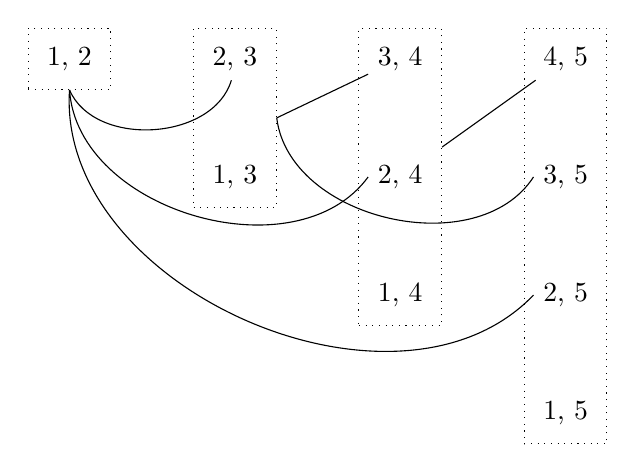
\begin{tikzpicture}
\foreach \x/\y/\z in {1/2/A, 1/3/B, 2/3/C, 1/4/D, 2/4/E, 3/4/F, 1/5/G, 2/5/H, 3/5/I, 4/5/J} {
  \node at (2.1*\y-2.1, 1.5*\x+1.5-1.5*\y) (\z) {\x, \y};
}
\node[draw,dotted,fit=(A)] (2) {};
\node[draw,dotted,fit=(B) (C)] (3) {};
\node[draw,dotted,fit=(D) (E) (F)] (4) {};
\node[draw,dotted,fit=(G) (H) (I) (J)] (5) {};
\draw (C) to [bend left = 70] (2.south);
\draw (E.west) to [bend left = 70] (2.south);
\draw (F) -- (3.east);
\draw (H.west) to [bend left = 70] (2.south);
\draw (I.west) to [bend left = 70] (3.east);
\draw (J) -- (4);
\end{tikzpicture}
\caption{The RMP for $S_{5, 2}$. Here, an edge means that we have all edges from the stable set on the left to the vertex on the right. Observe that every transversal is a forest, however we can form every graph on 4 vertices as a transversal minor.}
\end{figure}


Our goal is now to show that right extension preserves $\chi$-boundedness. We will express our result in the language of ordered graphs (graphs with a total order on vertices). An RMP for an ordered graph must respect the order, that is the parts of the partition must consist of consecutive vertices. The following result is not used in the proof that bounded twin-width graphs are \pcb, but it could be useful in other context and its proof is similar to a later argument.  
\begin{proposition}\label{prop:chibound} If $\mathcal{C}$ is a  $\chi$-bounded class of ordered graphs, then $RM(\mathcal{C})$ is $\chi$-bounded.
\end{proposition}

The proof of Proposition~\ref{prop:chibound} is heavily based on the following lemma about the clique number. Given an ordered graph $G$ and an RMP ${\mathcal P}=(V_1, \ldots, V_k)$, we denote by $G/\cal P$ the ordered graph obtained by contracting all parts of $\cal P$, i.e. $G / \{V_1, \ldots, V_k\}$. This is a particular transversal minor of $G$, with the property that $\chi (G) \leq \chi (G/{\cal P})$. 
A class $\cal C$ of ordered graphs is \emph{$h$-free} if it does not contain some ordered graph on $h$ vertices.

\begin{lemma} There exists a function $\phi$ such that for every $h$-free class $\cal C$ and every ordered graph $G$ with a $\cal C$-right module partition $\cal P$, we have $\omega (G/{\cal P})\leq \phi (\omega (G),h)$
\end{lemma}

\begin{proof}
    The proof is by induction on $\omega :=\omega(G)$ and $h$. 
    If $h=1$ or $\omega =1$ then $G$ is edgeless, so we can set $\phi(x,1)=\phi(1,y)=1$. 
    Now, $\omega \geq 2$ and $h \geq 2$, and we assume that we proved the existence of $\phi(\omega - 1, h)$ and $\phi(\omega, h-1)$.
    We denote $\mathcal{P} = (V_1, \ldots, V_k)$ and consider an ordered graph $H$ on vertices $v_1,\dots ,v_h$ which is not in $\cal C$. Observe that we can restrict ourselves to the case where $G/{\cal P}$ is a clique, as we can only consider a maximal clique of $G/{\cal P}$.
    
    Thus, for every $i < j \in [k]$, there is an edge between $V_i$ and $V_j$.
    Let $D_k$ be a subset of $V_k$ of minimal size such that there is an edge between $V_i$ and $D_k$ for every $i < k$. By minimality of $D_k$, for every $d \in D_k$ there exists $i_d \in [k-1]$ such that there is an edge between $V_{i_d}$ and $d$ (and thus $d$ dominates $V_{i_d}$) but no edge between $V_{i_d}$ and $D_k \setminus \{d\}$. We consider two cases depending on the size of $D_k$. 
    
    \begin{enumerate}
        \item If $|D_k| > \phi(\omega, h-1)+1$, we show that we reach a contradiction. Select some $x\in D_k$ and consider the set $\cal P '$ of $|D_k|-1$ parts $V_{i_d}$ as defined above, except for the part $V_{i_x}$ which is not selected in $\cal P '$. Since $G/\cal P'$ is a clique of size at least $\phi(\omega, h-1)+1$, it follows by induction that $(G[\cup {\cal P'}],\cal P')$ contains all ordered graphs of size $h-1$ as transversal minors. In particular, the ordered graph $H'=H\setminus v_h$ is a transversal minor of $\cal P '$.
        If $v_h$ is isolated in $H$, we reach a contradiction since $H'\cup x$ is isomorphic to $H$ and is a transversal minor of $(G,\cal P)$. Otherwise, observe that one can extend $H'$ in all possible ways as a transversal minor of $\cal P$ by selecting some vertices in $D_k$. Indeed, every $V_{i_d}$ corresponds to a vertex $d$ in $D_k$ which is only joined to $V_{i_d}$. We can then select vertices in $D_k$ to extend $H'$ to $H$, a contradiction.
        
        \item If $|D_k| \leq \phi(\omega, h-1)+1$. For $d \in D_k$, let $S_d$ be the set of neighbours of $d$ in $G$. In particular, $\omega(G[S_d]) \leq \omega - 1$. Furthermore, $\mathcal{P}$ induces by restriction a $\mathcal{C}$-RMP $\mathcal{P}_d$ of $G[S_d]$. We then have $\omega(G[S_d]/\mathcal{P}_d) \leq \phi(\omega - 1, h)$. By taking the union over all $d \in D_k$, we deduce $\omega(G/\mathcal{P}) \leq \phi(\omega - 1, h) \cdot (\phi(\omega, h-1) +1)+ 1$ (the additional +1 stands for the last class $V_k$ which is not dominated).
        
    
        
    \end{enumerate}

Therefore, we can choose $\phi(\omega, h) = \phi(\omega - 1, h) \cdot (\phi(\omega, h-1) +1)+ 1$.
\end{proof}

We are now ready to prove Proposition~\ref{prop:chibound}. If $\cal C$ has a $\chi$-bounding function $f$, by the fact that the class of all graphs is not $\chi$-bounded, there is a graph $H$ of size $h$ which is not in $\cal C$. Consider now any graph $G$ in $RM(\cal C)$ with clique number $\omega$ and $\mathcal{C}$-RMP $\cal P$. We have $$\chi (G)\leq \chi (G/{\cal P})\leq f(\omega (G/{\cal P}))\leq f(\phi(\omega(G),h)).$$

Therefore the function $f(\phi(\omega(G),h))$ is $\chi$-bounding for $RM(\cal C)$. This approach does not provide a polynomial bound if the class $\cal C$ is polynomially $\chi$-bounded. We could not prove (or disprove) that polynomial $\chi$-boundedness is preserved by RMP. However, this is the case when the twin-width of $\mathcal{C}$ is bounded, as shown in the following section. 
\section{Twin-width and almost-mixed minors}
  
  We recall here some definitions and results related to twin-width. For a more intuitive and pedestrian introduction, see~\cite{BKTW21}. We adopt here the matrix point of view of twin-width, where every graph $G$ is represented via its symmetric adjacency matrix $(a_{u,v})$ where $u,v$ are over couples of vertices. The entry $a_{u,v}$ is 1 if $uv$ is an edge, 0 if $uv$ is not an edge, and $*$ if $u=v$. The addition of the $*$ symbol slightly simplifies some technicalities, but is not necessary for the argument.
  
    A $01*$-matrix is \emph{horizontal} if all its rows are constant. It is \emph{vertical} if all its columns are constant. It is \emph{constant} if it is both horizontal and vertical. It is \emph{mixed} if it is neither horizontal nor vertical, or if it has at least 2 rows and 2 columns and contains a $*$ entry.
A \emph{corner} in a matrix $M$ is a mixed $2 \times 2$ submatrix of $M$.


\begin{lemma}[\cite{BKTW21}]\label{lem:corner}
 A matrix is mixed if and only if it contains a corner.
\end{lemma}

   Let $M$ be a matrix. 
    A \emph{row partition} of $M$ is a partition of the rows of $M$ in which each part of the partition consists of consecutive rows. We define \emph{column partitions} in a similar way. 
    A \emph{division} $\mathcal{D}$ of $M$ is a pair $(\mathcal{R}, \mathcal{C})$ where $\mathcal{R}$ is a row partition of $M$ and $\mathcal{C}$ is a column partition of $M$. If $\mathcal{R}$ and $\mathcal{C}$ both have the same number of parts, say $k$, we say that $(\mathcal{R}, \mathcal{C})$ is a \emph{$k$-division} of $M$. In this case, we index the row blocks and the column blocks of $\mathcal{D}$ with integers from $[k]$ in the natural order of the blocks. 
    If $\mathcal{D}$ is a $k$-division of $M$, for $i, j \in [k]$, we denote by $\mathcal{D}[i, j]$ the intersection of the $i$-th row block with the $j$-th column block, which we call a \emph{zone} of $\mathcal{D}$.  If $R_i\in \mathcal{R}$ and $C_j\in\mathcal{C}$, we also adopt the notation $[R_i,C_j]$ for the zone $\mathcal{D}[i, j]$. It is a contiguous submatrix of $M$.
    
    We say that a zone of a matrix is \emph{mixed} if it is mixed as a submatrix.
    If $M$ is symmetric, we say that a division $(\mathcal{R}, \mathcal{C})$ is \emph{symmetric} if $\mathcal{R}$ and $\mathcal{C}$ partition rows and columns in the same way (i.e. $\mathcal{R}$ is the transpose of $\mathcal{C}$).
    
    Let $M$ be a matrix and $\mathcal{D}$ be a $d$-division of $M$. We say that $\mathcal{D}$ is a \emph{$d$-mixed minor} if each zone of $\mathcal{D}$ is mixed. If $M$ does not have any $d$-mixed minor, we say that $M$ is \emph{$d$-mixed free}. The twin-width parameter and mixed-minor freeness are functionally equivalent. In particular, it was shown in \cite{BKTW21} that if a graph has twin-width at most $d$, it has a vertex ordering for which the adjacency matrix of $G$ is $f_d$-mixed free for some constant $f_d$.


    We also recall the following result, which is a direct consequence of the Marcus-Tardos theorem, see \cite{MT04}:

\begin{theorem}\label{th:marcustardos}
    For every positive integer $d$, there is a constant $mt_d$ such that for every $d$-mixed free matrix $M$ and every $k$-division of $M$, the number of mixed zones is at most $mt_d \cdot k$
\end{theorem}
   
As we will perform some operations on our graphs (such as deleting edges and contracting subsets of vertices), we show in the next results how mixed zones are affected. Let $M$ be a $01*$-matrix (not necessarily an adjacency matrix) with exactly two row blocks $R,R'$ and two columns blocks $C,C'$, each of size at least two. 

\begin{lemma}\label{lem:4corner}
If all four zones of $M$ are mixed, there is a corner intersecting all zones.
\end{lemma}

\begin{proof}
This is clear if $M$ contains a $*$. Consider a non constant row $r$ in $[R,C]$ and a non constant column $c'$ in $[R',C']$. Let $e$ be the entry $(r,c')$. Let $c\in C$ such that $e\neq (r,c)$ and $r'\in R'$ such that $e\neq (r',c')$. Now $\{r,r'\},\{c,c'\}$ is a corner.
\end{proof}

The \emph{contraction} $M'=M/\{R,R';C,C'\}$ is the $2\times 2$-matrix obtained by keeping a single value $x$ for each of the 4 zones, with the following rule: $x$ is the maximum value of the zone according to the order $0<1<*$. Thus, we get $*$ as soon as there exists a $*$, and we get $0$ only if the zone is full $0$.

\begin{lemma}\label{lem:contract}
If $M'$ is mixed, then $M$ is mixed.
\end{lemma}

\begin{proof}
This is clear if $M'$ (thus equivalently $M$) contains a $*$. Let us assume by contrapositive that $M$ is non-mixed. If $M$ is vertical (resp. horizontal), then observe that $M'$ is also vertical (resp. horizontal).
\end{proof}
 
 We keep the same notations as before, and assume moreover that none of the four zones of $M$ is mixed (in particular $M$ has no value $*$). The \emph{horizontal-deletion} $M_H$ of $M$ is the matrix obtained from $M$ by setting all values to 0 in each zone which is not vertical (or equivalently each zone which is horizontal and non-constant). We similarly define the \emph{vertical-deletion} $M_V$.
 
\begin{lemma} \label{lem:deletion}
If $M_H$ is mixed, then $M$ is mixed.
\end{lemma}

\begin{proof}
 Let us assume by contrapositive that $M$ is non-mixed. By assumption, there is no $*$ in  $M_H$. If $M$ is vertical, then observe that $M_H$ is also vertical. Now if $M$ is horizontal, note that the zones $R,C$ and $R,C'$ are either both set to 0 (if they are not vertical), or both left as in $M$. In both cases the rows of $R$ in $M_H$ are constant. The same applies to $R'$, so $M_H$ is horizontal. 
\end{proof}


Here is the key-definition of \cite{PS22}.   A $d$-division $\mathcal{D}$ of a matrix $M$ is a \emph{$d$-almost mixed minor} if for every $i \neq j \in [d]$, the zone $\mathcal{D}[i, j]$ is mixed. If $M$ does not have any $d$-almost mixed minor, we say that $M$ is \emph{$d$-almost mixed free}. By extension, a graph is \emph{$d$-almost mixed free} if we can order its vertices in such a way that its adjacency matrix is $d$-almost mixed free.

Observe that every $d$-almost mixed free matrix is also $d$-mixed free. Conversely, every $d$-mixed free matrix is also $2d$-almost mixed free. Indeed, if $M$ has a $2d$-almost mixed minor, then merging the first $d+1$ row blocks, and the last $d+1$ column blocks gives a $d$-mixed minor of $M$. Note that every submatrix of a $d$-(almost) mixed free matrix is also $d$-(almost) mixed free, hence every subgraph of a $d$-almost mixed free graph is also $d$-almost mixed free. 

Let $G$ be a graph with an RMP $\mathcal{P} = (V_1, \ldots, V_k)$. We say that $(G,\mathcal{P})$ is \emph{$d$-almost mixed free}, if for every coarsening $\cal P'$ of $\cal P$ into $d$ parts $(V'_1, \ldots, V'_d)$, where each $V'_i$ consists of consecutive parts of $\cal P$, some zone $[V'_i,V'_j]$, where $i\neq j$, is not mixed in the adjacency matrix of $G$. Note that we only speak here of restrictions on symmetric divisions of $G$, which encompass much larger classes than bounded twin-width. 

\begin{lemma} If $(G,\cal P)$ is $d$-almost mixed free, then  $\omega (G/{\cal P})\leq \omega(G)^d$.
\end{lemma}

\begin{proof}
We write $\omega:=\omega(G)$ and denote $\mathcal{P} = (V_1, \ldots, V_k)$. Let $\phi$ such that $\omega(G/{\cal P}) \leq \phi(\omega, d)$. We have $\phi(\cdot, 1)=0$ (empty graph) and $\phi(1, \cdot) = 1$ (edgeless graph). We assume $\omega\geq 2$ and $d\geq 2$ and show that $\phi(\omega, d)= \phi(\omega-1, d)+\phi(\omega, d-1)+1$ upper bounds $\omega(G/{\cal P})$. We can restrict ourselves to a maximal clique of $G/{\cal P}$, so we can assume that there is an edge between $V_i$ and $V_j$ whenever $i < j \in [k]$.    

Let us consider the smallest $\ell$ such that $\omega(G[V_1\cup \dots \cup V_{\ell}])=\omega$. Denote by $Y$ the set $V_1\cup \dots \cup V_{\ell}$, and consider any $V_i$ where $i\geq \ell +1$. Note that $Y$ is not a module with respect to $V_i$, as some vertex in $V_i$ would dominate $Y$, hence forming a clique of size $\omega +1$ in $G$. Conversely, if $V_i$ is a module with respect to $Y$, since $\cal P$ is an RMP, and there exists an edge between all pairs of parts, $V_i$ would dominate $Y$, with the same contradiction.

Consider the graph $G'=G[V_{\ell+1}\cup \dots \cup V_{k}]$ and its RMP $\mathcal{P'} = (V_{\ell +1}, \ldots, V_k)$. We claim that $(G',\cal P')$ is $d-1$-almost mixed free, otherwise any $d-1$-almost mixed minor coarsening $(V'_1, \ldots, V'_{d-1})$ of $\mathcal{P'}$ could be extended to the $d$-almost mixed minor $(Y,V'_1, \ldots, V'_{d-1})$ of $(G,\cal P)$. 

Thus $k=\omega (G/\cal P)$ satisfies by induction that $k\leq \ell + \phi(\omega, d-1)$. And since the first $\ell -1$ parts do not contain a clique of size $\omega$, we have $k \leq \phi(\omega - 1, d) + 1 + \phi(\omega, d-1)= \phi(\omega, d)$. Setting  $\psi(\cdot,\cdot)=\phi(\cdot,\cdot)-1$, we have that $\psi (\omega,d)=\psi(\omega - 1, d) + \psi(\omega, d-1)$. Moreover, we both have $\psi (\omega,1)=-1$ and $\psi (1,d)=0$, so $\psi (\omega,d)\leq \binom{\omega + d - 2}{d-1}\leq \omega ^{d-1}$.
\end{proof}

\begin{proposition} \label{prop:RMPpcb} Let $\cal C$ be a class of graphs with polynomial $\chi$-bounding function $f(x)=x^c$. If $\cal P$ is a $\cal C$-RMP of $G$ such that $(G,\cal P)$ is $d$-almost mixed free, then $\chi (G)\leq \omega ^{cd}$.
\end{proposition}

\begin{proof}
   Since $\omega(G/{\cal P}) \leq \omega(G)^{d}$, we have $\chi(G)\leq \chi(G/{\cal P})\leq \omega(G/{\cal P})^c\leq \omega(G)^{cd}$.
\end{proof} 
\section{Polynomial $\chi$-boundedness of bounded twin-width graphs}

By Lemma~\ref{lem:mixedtww}, in order to prove our main result, Theorem~\ref{th:BT}, we just have to show that the class of $d$-mixed free graphs is polynomially $\chi$-bounded. Since mixed freeness is functionally
equivalent to almost mixed freeness, we only consider this last notion.


To prove that a class $\cal C$ is \pcb, a strategy is to show that every graph $G$ of $\cal C$ has a vertex-partition or an edge-partition into a bounded number of graphs, each of them belonging to some known \pcb~class $\cal C '$. We will use this argument several times here.

\begin{theorem}\label{thm:damf-pcb} The class of $d$-almost mixed free graphs is \pcb.
\end{theorem}

\begin{proof}
The proof is by induction on $d$. For $d=2$, if $G$ has a 2-almost mixed free adjacency matrix, $G$ is a cograph (see \cite{PS22}), hence $G$ is perfect so the property holds. Now, let $d \geq 3$ and consider a graph $G$, which is $d$-almost mixed free with respect to the vertex ordering $v_1,\ldots ,v_n$. We first partition the set of vertices $V' =\{v_2,\dots, v_{n-1}\}$ into four subsets $V'_{00},V'_{01},V'_{10},V'_{11}$ according to their neighbourhood in $\{v_1,v_n\}$. For instance, $V'_{01}=(V'\setminus N(v_1))\cap N(v_n)$. It suffices to show that all four graphs $G[V'_{ij}]$ belong to some \pcb~class. Hence, without loss of generality, we can assume that $V'$ is a module in $G$. 
    We now consider the delayed decomposition tree $(T_d,g)$ of $G':=G[V']$ and consider the class $\cal C$ containing all $g(x)$ and their induced subgraphs. By Corollary~\ref{cor:delay}, we just have to show that $\cal C$ is \pcb. The graphs $g(x)$ are obtained by starting from an interval $I=\{v_s,\dots, v_t\}$ of vertices of $G'$, partitioning it into local modules $L_1,\dots, L_k$, and then partitioning each local module into local submodules. Let $H$ be the graph we obtain from $G[I]$ by removing all edges inside all local modules $L_i$. Note that $H$ can also be obtained by substituting the vertices of $g(x)$ by stable sets. This does not change $\chi$ and $\omega$. Therefore, to show that $\mathcal{C}$ is \pcb, it suffices to prove the following.

\begin{claim} Let $I=\{v_s,\dots, v_t\}$ be any interval of vertices of $G'$. Consider its partition into local modules $L_1,\dots, L_k$ and denote by $H$ the graph on vertex set $I$ obtained from $G[I]$ by deleting the edges inside the local modules. Then, $H$ is a bounded (vertex and edge) union of graphs from hereditary \pcb~classes.
\end{claim}

Note that the claim holds when $I$ is a non trivial module since it is cut into two parts. Indeed, in this case $H$ is bipartite and thus $\chi$-bounded by 2. Assume now that we have local modules $L_1,\dots ,L_k$, and consider all pairs $i<j$ such that $G[L_i,L_j]$ is mixed (call \emph{mixed pairs}). The $L_i$'s form a $k$-division of the adjacency matrix of $G[I]$, which is $d$-mixed free. Thus, by Theorem \ref{th:marcustardos}, the graph $R$ on vertex set $[k]$ whose edges correspond to mixed pairs has at most $\frac{mt_d}{2} \cdot k$ edges. In particular, $R$ can be vertex-colored into $(mt_d+1)$ classes. In other words, one can partition the set of local modules into $(mt_d+1)$ subsets, in which local modules are not pairwise mixed. We denote by $L'$ such a subset of local modules. To prove our claim, we just have to show that $H':=H[L']$ belongs to a \pcb~class of graphs.

Observe that for every $i<j$ and $L_i,L_j\in L'$, we have that $L_i$ is a module in $H[L_i\cup L_j]$ (denoted $L_i\rightarrow L_j$) or $L_j$ is a module in $H[L_i\cup L_j]$, that is $L_j\rightarrow L_i$. Note that if we both have $L_j\rightarrow L_i$ and $L_i\rightarrow L_j$, we have all edges or no edge between $L_i$ and $L_j$. We now define two subgraphs $H'_{\rightarrow}$ and $H'_{\leftarrow}$ of $H'$: in $H'_{\rightarrow}$ we only keep the edges of $H'$ between pairs $L_i\rightarrow L_j$ where $i<j$, and in $H'_{\leftarrow}$ we only keep the edges of $H'$ between pairs $L_i\leftarrow L_j$ where $i<j$.
Note that $H'=H'_{\rightarrow}\cup H'_{\leftarrow}$, and thus we just have to show that (for instance) $H'_{\rightarrow}$ belongs to a \pcb~class of graphs.

The graph $H'_{\rightarrow}$ with the partition $L'$ is a right module partition. Note that the same holds for $H'_{\leftarrow}$ if we reverse the order of the local modules. 
We further partition $H'_{\rightarrow}$: let us say that a local module $L_i$ is \emph{left} if $i>1$ and there is a vertex $v_j$ among $v_1,v_2,\dots,v_{s-1}$ (i.e. to the left of $I$) which distinguishes $L_{i-1}$ from $L_i$. Precisely, $v_j$ is not joined in the same way to the last vertex of $L_{i-1}$ and to the first of $L_i$. If $L_i$ (with $i>1$) is not left, then it is \emph{right} (and indeed some vertex $v_j$ to the right of $I$ distinguishes $L_{i-1}$ from $L_i$). We neglect $L_1$ in this definition (it only adds 1 to the chromatic number of $H'$). We now partition $L'$ into $L'_{ri}$ containing all right local modules $L_i$ of $L'$, and $L'_{le}$ containing the left local modules. Again, by vertex partition, we just have to show that the RMP $H'_{\rightarrow,ri}$ which is the induced restriction of $H'_{\rightarrow}$ to $L'_{ri}$ is \pcb. To apply Proposition~\ref{prop:RMPpcb}, we first show that the transversal minors of  $(H'_{\rightarrow,ri},L'_{ri})$ are $d-1$-almost mixed free, which by induction implies that they are \pcb. Then we argue that $(H'_{\rightarrow, ri},L'_{ri})$ has no large almost mixed minor. It suffices here to show that it is $2d$-almost mixed free. These are our last results.

\begin{claim}[\cite{PS22}]\label{claim:twwreduction}
    Every transversal minor of  $(H'_{\rightarrow,ri},L'_{ri})$ is $d-1$-almost mixed free.
\end{claim}

\begin{proof}
Assume for contradiction that we can find a sequence of local modules $L'_1,\dots ,L'_t$ in $L'_{ri}$, each of them containing a non empty subset of vertices $W_1,\dots ,W_t$, such that the graph $Q=H'_{\rightarrow,ri}/\{W_1,\dots ,W_t\}$ has a $d-1$-almost mixed minor. The vertices of $Q$ are denoted $W=\{w_1,\dots ,w_t\}$, where $W_i$ is contracted to $w_i$. Moreover, there exist two partitions of $W$ into consecutive blocks of vertices $(R_1,\dots ,R_{d-1})$ and $(C_1,\dots ,C_{d-1})$ such that $Q$ is mixed on the zone $[R_i,C_j]$ whenever $i\neq j$ (thus all $R_i$ and $C_j$ have size at least 2). We now show how to "lift" these partitions to $G$ in order to get a contradiction.

Consider any partition ${\cal R}'=(R'_1,\dots ,R'_{d-1})$ of $I$ (where parts consist of consecutive local modules) satisfying that $w_i\in R_j$ implies $L'_i \subseteq R'_j$. Similarly ${\cal C}'=(C'_1,\dots ,C'_{d-1})$ partitions $I$ and $w_i\in C_j$ implies $L'_i \subseteq C'_j$. We now extend the partitions ${\cal R}',{\cal C}'$ of $I$ to the whole vertex set $V$ of $G$ by first setting $R'_1:=R'_1\cup \{v_1,\dots ,v_{s-1}\}$ and $C'_1:=C'_1\cup \{v_1,\dots ,v_{s-1}\}$, and then adding a new part $\{v_{t+1},\dots ,v_{n}\}=R'_d=C'_d$ to both ${\cal R}'$ and ${\cal C}'$. These new partitions are called ${\cal R}$ and ${\cal C}$. Observe that if we were working with $H'_{\rightarrow,le}$, we would have added the part $R'_0=C'_0=\{v_1,\dots ,v_{s-1}\}$ to both ${\cal R}'$ and ${\cal C}'$ and extended the parts $R'_{d-1}$ and $C'_{d-1}$ by adding $\{v_{t+1},\dots ,v_{n}\}$. 


We now show that ${\cal R}$ and ${\cal C}$ form a $d$-almost mixed minor for $G$, which will be our contradiction. We need to focus on two points: the added parts $R'_d,C'_d$ should be mixed with respect to the others, and the original mixed zones $[R_i,C_j]$ of $Q$ should yield mixed zones $[R'_i,C'_j]$ of $G$. We separate the two arguments:
\begin{itemize}
    \item Consider first some zone $[R'_i,C'_d]$ where $i<d$ (similar argument for $[R'_d,C'_i]$). By the fact that $R_i$ contains two vertices $w_a,w_b$, the part $R'_i$ contains the right local modules $L'_a,L'_b$ (where $a<b$). Focus now on the vertex $v_j$ which is the first vertex of $L'_b$, and note that $v_{j-1}\in R'_i$ since $L'_a\subseteq R'_i$. Since $L'_b$ is a right local module, there exists $v_k$, where $k>t$ such that $v_k$ is differently joined to $v_{j-1}$ and $v_j$. Recall that $v_n$ is joined in the same way to $v_{j-1}$ and $v_j$. Since $v_{j-1},v_j\in R'_i$ and $v_k,v_n\in C'_d$, they witness the fact that $[R'_i,C'_d]$ is mixed. 
    \item Now, consider any zone $[R'_i,C'_j]$ where $i,j<d$ and $i\neq j$. If the zone $[R_i,C_j]$ contains a $*$ (i.e. some $w_a$ both belongs to $R_i$ and $C_j$), then $[R'_i,C'_j]$ also contains a $*$. Otherwise, by Lemma \ref{lem:corner}, $R_i$ contains two vertices $w_a,w_b$ and $C_j$ contains two vertices $w_c,w_d$ such that $\{w_a,w_b\},\{w_c,w_d\}$ is a corner. Moreover, since there is no $*$ value, we have $a<b<c<d$ or $c<d<a<b$. Without loss of generality, we assume $a<b<c<d$. By Lemma~\ref{lem:contract}, the restriction of the adjacency matrix of $H'_{\rightarrow,ri}$ on $[W_a\cup W_b,W_c\cup W_d]$ is mixed since its contraction is the corner $\{w_a,w_b\},\{w_c,w_d\}$. So the submatrix $[L'_a\cup L'_b,L'_c\cup L'_d]$ is also mixed.
    By definition of $H'_{\rightarrow,ri}$, if $L'_a$ (or $L'_b$) is not a module with respect to $L'_c$ (or to $L'_d$), then the zone $[L'_a,L'_c]$ is set to 0. In other words, the adjacency matrix of $H'_{\rightarrow,ri}$ restricted to $[L'_a\cup L'_b,L'_c\cup L'_d]$, is the horizontal-deletion of the adjacency matrix of $G$. Thus the zone $[R'_i,C'_j]$ is mixed by Lemma~\ref{lem:deletion}.
\end{itemize}
\end{proof}
\begin{claim}
    The pair $(H'_{\rightarrow,ri},L'_{ri})$ is $2d$-almost mixed free.
\end{claim}

\begin{proof}
    Assume for contradiction that we can find a coarsening $W'_1,\dots ,W'_{2d}$ of $L'_{ri}$ which forms a $2d$-almost mixed minor of $H'_{\rightarrow,ri}$. We now set $W_i=W'_{2i-1}\cup W'_{2i}$ for all $i=1,\dots ,d$. 
    By Lemma~\ref{lem:corner} every (mixed) zone $[W_i,W_j]$ with $i\neq j$ of $H'_{\rightarrow,ri}$ contains a corner $\{w_a,w_b\},\{w_c,w_d\}$.  By Lemma~\ref{lem:4corner}, we can assume that $w_a,w_b,w_c,w_d$ belong respectively to $W'_{2i-1},W'_{2i},W'_{2j-1},W'_{2j}$, hence to respective distinct local modules $L'_a,L'_b,L'_c,L'_d$.
    We assume without loss of generality that $i<j$, and thus $a<b<c<d$. 
    By definition of $H'_{\rightarrow,ri}$, if $L'_a$ (or $L'_b$) is not a module with respect to $L'_c$ (or to $L'_d$), then the zone $[L'_a,L'_c]$ is set to 0. In other words, the adjacency matrix of $H'_{\rightarrow,ri}$ restricted to $[L'_a\cup L'_b,L'_c\cup L'_d]$, is the horizontal-deletion of the adjacency matrix of $G$. Hence the zone $[W_i,W_j]$ is mixed in $G$ by Lemma~\ref{lem:deletion}. Thus $G$ restricted to $W_1,\dots ,W_d$ has a $d$-almost mixed minor, a contradiction.
\end{proof}
We can conclude the proof of Theorem~\ref{thm:damf-pcb} by using the two previous Claims and Proposition~\ref{prop:RMPpcb}.
\end{proof}

Theorem~\ref{th:BT} now follows from Lemma~\ref{lem:mixedtww} and Theorem~\ref{thm:damf-pcb}. From the previous proof, the order of magnitude for the $\chi$-bounding function of graphs with no $d$-almost mixed minor is $\omega^{d^{O(d)}}$.

\section{More on the $\chi$-boundedness of substitution-closure}\label{sec:subs}


The goal of this section is to provide a proof of the following theorem by slightly modifying the original argument of Chudnovsky, Penev, Scott and Trotignon~\cite{CPST13}.


\begin{theorem}\label{th:chibordec}
If $\cal C$ is hereditary and \pcb~with function $\chi \leq \omega^k$, then ${\cal C}_s$ is \pcb~with function $\chi \leq \omega^{2k+3}$
\end{theorem}

Given a class of graphs $\cal C$, a \emph{$\cal C$-tree-decomposition} is a pair $(T,g)$ in which $T$ is a rooted tree and $g$ is a function associating to every internal node $x$ of $T$ a graph $g(x)\in \cal C$ whose vertices are the children of $x$. The \emph{realization} $R(T,g)$ is the graph such that: 
\begin{itemize}
    \item its vertex set is the set of leaves $L$ of $T$
    \item two vertices $x,y\in L$ are joined by an edge if, given that $z$ is their closest ancestor in $T$ and $x',y'$ are the respective children of $z$ which are the ancestors of $x,y$, the edge $x'y'$ belongs to $g(z)$.
\end{itemize}

Given a class $\cal C$, we denote by ${\cal C}_s$ the class of all $R(T,g)$ where $(T,g)$ is a $\cal C$-tree-decomposition. For instance, if $\cal C$ is the class of cliques and independent sets, then  ${\cal C}_s$ is the class of cographs.
We say that $(T,g)$ is \emph{independent} if whenever $x, y$ are internal nodes of $T$ with the same parent $z$, then $xy$ is not an edge of $g(z)$. We denote by ${\cal C}_i$ the class of all $R(T,g)$ where $(T,g)$ is an independent $\cal C$-tree-decomposition. \\
Let $\cal C$ be a class of graphs, and $(T, g)$ be a $\cal C$-tree-decomposition. 
Let $u$ be any node of $T$ which is not the root, and let $v$ be the parent of $u$. We say that $u$ is \emph{isolated} in $T$ if it is isolated in $g(v)$. \\
The \emph{depth} $d(x)$ of a node $x$ of $T$ is the number of strict ancestors of $x$ in $T$ that are not isolated.
The \emph{depth} $d(T, g)$ of $(T, g)$ is the maximum depth of a leaf of $T$. 
Finally, if $G \in \mathcal{C}_s$, the \emph{depth} of $G$ is the minimum depth of a $\cal C$-tree-decomposition $(T, g)$ such that $G = R(T, g)$.

\begin{lemma}\label{lem:depth}
For every class $\cal C$, if $(T, g)$ is a $\mathcal{C}$-tree-decomposition of depth $d$, then $\omega(R(T, g)) \geq d + 1$.
\end{lemma}

\begin{proof} We consider a leaf $x$ with depth $d$. We denote by $y_1,\dots, y_d$ the non-isolated ancestors of $x$, and by $z_1,\dots, z_d$ their respective parents. We also denote by $w_1,\dots, w_d$ some respective children of $z_1,\dots, z_d$ such that $y_iw_i$ is an edge in $g(z_i)$. We now pick some leaves $x'_1,\dots ,x'_d$ which are respective descendants of $w_1,\dots, w_d$. Observe that $x,x'_1,\dots ,x'_d$ is a clique of $R(T, g)$.
\end{proof}

\begin{theorem}\label{th:inddec}
If $\cal C$ is \pcb~with function $\chi \leq \omega^k$, then ${\cal C}_i$ is \pcb~with function $\chi \leq \omega^{k+1}$
\end{theorem}

\begin{proof}
Let $G \in \mathcal{C}_i$. There exists an independent $\cal C$-tree-decomposition $(T, g)$ such that $G = R(T, g)$. By Lemma \ref{lem:depth}, we have $\omega(G) \geq d(T, g) + 1$. For every internal node $x$, we have $g(x) \in \cal C$ and $\omega(g(x)) \leq \omega(G)$, thus $g(x)$ is $\omega(G)^k$-colorable. For every internal node $x$, let $\alpha_x$ be an $\omega(G)^k$-coloring of $g(x)$. Let $v$ be any vertex of $G$ (equivalently $v$ is a leaf of $T$). If $T$ has only one node, then $G$ is the graph on a single vertex, so $G$ is $\omega(G)^{k+1}$-colorable. Otherwise, let $x$ be the parent of $v$ in $T$. We set $c(v) = (d(v), \alpha_x(v))$, where $d(v)$ is the depth of $v$ in $(T, g)$. \\
We claim that $c$ is a proper $\omega(G)^{k+1}$-coloring of $G$. First, for every vertex $v$ of $G$, we have $0 \leq d(v) \leq d(T, g) \leq \omega(G) - 1$, so we indeed use at most $\omega(G)^{k+1}$ colors. Then, let $uv$ be an edge of $G$. Let $z$ be the closest ancestor of $u$ and $v$ in $T$, and $u', v'$ be the respective children of $z$ which are the ancestors of $u, v$. The edge $u'v'$ belongs to  $g(z)$. Since $(T, g)$ is an independent $\cal C$-tree-decomposition, this implies that either $u'$ or $v'$ is a leaf (or both). If they are both leaves, we have $u = u'$ and $v = v'$, therefore $u$ and $v$ are children of $z$ which are adjacent in $g(z)$. Thus, $\alpha_z(u) \neq \alpha_z(v)$ so $c(u) \neq c(v)$. If only one of $u', v'$ is a leaf, say $u'$, then we have that $v'$ is a strict ancestor of $v$ which is not isolated, so $d(v) > d(v') = d(u') = d(u)$ hence $c(u) \neq c(v)$. 
\end{proof}

\begin{proof} We now prove \ref{th:chibordec} by induction on the depth of $G$. \\
If $G$ has depth 0, then $G$ is a disjoint union of graphs of $\cal C$, so $\chi(G) \leq \omega(G)^k \leq \omega(G)^{2k+3}$.
Now, suppose $G$ has depth 1. By a previous lemma, we have $\omega(G) \geq 2$. We can assume that $G$ is connected since we can deal with each connected component separately. Then $G$ can be obtained by starting from a graph $G_0 \in \mathcal{C}$ on vertex set $v_1, \ldots, v_n$ and substituting each $v_i$ by a graph $G_i \in \mathcal{C}$. Let $X = \{v_i, \omega(G_i) \leq \sqrt{\omega(G)}\}$ and $Y = V(G_0) \setminus X$. Let $G_X$ be the subgraph of $G$ induced by the leaves which are descendant of nodes of $X$ and $G_Y$ be the graph induced on the other vertices. The graph $G_X$ is obtained by substituting graphs of $\mathcal{C}$ of clique number at most $\sqrt{\omega(G)}$ inside a graph of $\mathcal{C}$ of clique number at most $\omega(G)$. Hence, $G_X$ can be colored with at most  $\omega(G)^{1.5k}$ colors (consider the product of the colorings). Similarly, the graph $G_Y$ is obtained by substituting graphs of $\mathcal{C}$ of clique number at most $\omega(G)$ inside a graph of $\mathcal{C}$ of clique number at most $\sqrt{\omega(G)}$ so it can be colored with at most  $\omega(G)^{1.5k}$ colors. Hence $G$ can be colored with $2\omega(G)^{1.5k} \leq \omega(G)^{1.5k+1} \leq \omega(G)^{2k+3}$ colors. \\

Now, suppose that $G$ has depth at least 2. Thus, $\omega(G) \geq 3$. Let $(T, g)$ be a $\mathcal{C}$-tree-decomposition of $G$. For every node $x$ of $T$, let $T_x$ be the subtree of $T$ that is rooted in $x$, $g_x$ be the restriction of $g$ to the internal nodes of $T_x$, and $G_x = R(T_x, g_x)$. Finally, let $X = \{x, \omega(G_x) > \omega(G)/2\}$. Note that if $z$ is the parent of $x$ in $T$, then $G_x$ is an induced subgraph of $G_z$, so if $x \in X$, then we also have $z \in X$. In particular, $T[X]$ is a subtree of $T$. Let $C(X)$ be the set of children of an element of $X$ in $T$ and $Y = X \cup C(X)$. Let $T' = T[Y]$. $T'$ is also a subtree of $T$. Let $g'$ be the restriction of $g$ to the internal nodes of $T'$, and let $H = R(T', g')$. Note that $H$ is an induced subgraph of $G$ so $\omega(H) \leq \omega(G)$. Now, suppose $x, y$ are internal nodes of $T'$ with the same parent $z$. Then, $x, y \in X$ so $\omega(G_x), \omega(G_y) > \omega(G)/2$. Thus, $x$ and $y$ cannot be adjacent in $g'(z)$ otherwise we would have $\omega(H) > \omega(G)$. This means that $(T', g')$ is an independent $\mathcal{C}$-tree-decomposition of $H$, so $H \in \mathcal{C}_i$. Thus, $H$ is $\omega(H)^{k+1} \leq \omega(G)^{k+1}$-colorable. \\
Let $v_1, \ldots, v_n$ be the vertices of $H$. We have that $G$ can be obtained by substituting each $v_i$ by some $G_{v_i} \in \mathcal{C}_s$. We can assume that $G$ is connected since we can deal with each connected component separately. Thus, we get that for every $i \in [n]$, $d(G_{v_i}) < d(G)$ (where $d$ stands for the depth). Futhermore, if $v_i$ is a vertex of $H$, it means that it is a leaf of $T'$. Indeed, since $\omega(G) \geq 3$, if $v_i \in X$ then $\omega(G_{v_i}) \geq 2$ so $v_i$ has children in $T$. Thus, $v_i \notin X$, which means $\omega(G_{v_i}) \leq \omega(G)/2$. Let $\omega_i = \omega(G_{v_i})$. By induction hypothesis, we have $\chi(G_{v_i}) \leq \omega_i^{2k+3}$. \\
Let $m = \lfloor\log(\omega(G))\rfloor$. For $j \in [m]$, let $V_j = \{v_i: \frac{\omega(G)}{2^{j+1}} < \omega_i \leq \frac{\omega(G)}{2^j}\}$. Note that the $V_j$'s partition  $\{v_1, \ldots, v_n\}$. For $j \in [m]$, let $H_j = H[V_j]$ and $G_j$ be the corresponding induced subgraph of $G$. 

If $j \in [m]$ and $v_i \in V_j$ then $\omega_i > \frac{\omega(G)}{2^{j+1}}$ so $\omega(H_j) \leq 2^{j+1}$. Thus, $\chi(H_j) \leq 2^{(j+1)(k+1)}$ because $H_j$ is an induced sugraph of $H\in \mathcal{C}_i$. Thus, we have $\chi(G_j) \leq 2^{(j+1)(k+1)} \cdot \left(\frac{\omega(G)}{2^{j}}\right)^{2k+3}$ (by doing the product of the colorings). Now, let's color separately each $V_j$ with a different palette. The number of colors used is: \begin{align*}
    \sum_{j=1}^m \chi(G_j) &\leq \sum_{j = 1}^m 2^{(j+1)(k+1)} \cdot \left(\frac{\omega(G)}{2^{j}}\right)^{2k+3} \\
                            &= 2^{k+1} \omega(G)^{2k+3} \sum_{j = 1}^m 2^{-j(k+2)} \\
                            &\leq 2^{k+1} \omega(G)^{2k+3} \frac{2^{-(k+2)}}{1-2^{-(k+2)}} \\
                            &\leq \omega(G)^{2k+3} \times \frac{2^{k+2}}{2(2^{k+2} - 1)} \\
                            &\leq \omega(G)^{2k+3}
\end{align*}
\end{proof}
\section{Mixed extensions}

We conclude with another type of class extension which preserves  $\chi$-boundedness. Given an ordered graph $G$ with vertex ordering  $v_1,\dots ,v_n$ (denoted by $<$), we only ask here that the restriction to "mixed parts" of $G$ are $\chi$-bounded. Precisely, given a class $\cal C$ of graphs, we say that $(G,<)$ is a \emph{$\cal C$-mixed extension} if for every partition $\cal P$ into intervals $I_1,\dots ,I_k$, the subgraph $\text{Mix}(G,<,\cal P)$ of $G$ in which we only keep edges between intervals $I_s,I_t$ for which $I_s,I_t$ is mixed, belongs to $\cal C$. The class of graphs $G$ admitting a vertex-ordering $<$ such that $(G,<)$ is a $\cal C$-mixed extension is denoted by ME$(\cal C)$.

Observe that graphs with twin-width at most $d$ are mixed extensions of the class of graphs with chromatic number at most $f(d)$. To see this, observe that they admit vertex-orderings with no large mixed-minors, hence the Marcus-Tardos theorem implies that every partition $\cal P$ has a linear number of mixed zones. So $\text{Mix}(G,<,\cal P)$ has bounded chromatic number by degeneracy. Hence the fact that bounded twin-width graphs are $\chi$-bounded is a particular case of the following result (whose proof mimics the one of Proposition~\ref{prop:RMPpcb}):



\begin{theorem}\label{th:chimix}
If $\cal C$ is $\chi$-bounded, then ME$(\cal C)$ is $\chi$-bounded.
\end{theorem}

\begin{proof} Assume that all graphs $H$ in $\mathcal{C}$ satisfy $\chi(H)\leq f(\omega (H))$. Consider $G\in \cal C$ with clique number $\omega$ and assume that we have already proved that the chromatic number of every graph in $ME(\mathcal{C})$ with smaller value of $\omega$ is at most $c$. Consider $<$, a vertex ordering $v_1,\dots ,v_n$ of $G$ such that $(G,<)$ is a $\cal C$-mixed extension. Pick a smallest initial interval $I_1=v_1,\dots ,v_{i_1}$ such that $G[I_1]$ has a clique of size $\omega$. Then pick a smallest interval $I_2=v_{i_1+1},\dots ,v_{i_2}$ such that $G[I_2]$ has a clique of size $\omega$, otherwise pick all remaining vertices. Continue the process to get a partition $\cal P$ into intervals $I_1,\dots ,I_k$. Observe that if there is an edge between $I_s$ and $I_t$, where $s<t<k$, then $I_s,I_t$ is mixed, otherwise one of the intervals would be a module with respect to the other, and we would find a clique of size $\omega +1$. Therefore the chromatic number of $G$ is at most $(c+1)f(\omega )+c+1$ since $\chi(G[I_k])\leq c+1$ and  $G[I_1\cup \dots \cup I_{k-1}]$ is the edge union of two graphs, one of chromatic number at most $c+1$ inside the $I_i$'s, and one of chromatic number at most $f(\omega)$ across the $I_i$'s.
\end{proof}



%%% AUTHOR: optional acknowledgments here
% \section*{Acknowledgments} %%  you may comment this out if no Ackno
% The authors are grateful to the anonymous reviewers for finding
% a bug in the main result.

%%% AUTHOR:
%%% Bibliography goes here. Note that the arXiv cannot process bibtex
%%% or biber bibliographies.  Example of acceptable bibliograpy format:
\bibliographystyle{amsplain}
\begin{thebibliography}{10}

\bibitem{BP19}
Marthe Bonamy and Micha\l{} Pilipczuk.
\newblock Graphs of bounded cliquewidth are polynomially $\chi$-bounded.
\newblock {\em Advances in Combinatorics}, (8):21pp, 2020.

\bibitem{BBDGT23}
\'Edouard Bonnet, Romain Bourneuf, Julien Duron, Colin Geniet, Stéphan
  Thomassé, and Nicolas Trotignon.
\newblock A tamed family of triangle-free graphs with unbounded chromatic
  number.
\newblock 2023.

\bibitem{BGKTW21}
\'{E}douard Bonnet, Colin Geniet, Eun~Jung Kim, St\'{e}phan Thomass\'{e}, and
  R\'{e}mi Watrigant.
\newblock {Twin-width III: Max Independent Set, Min Dominating Set, and
  Coloring}.
\newblock In Nikhil Bansal, Emanuela Merelli, and James Worrell, editors, {\em
  48th International Colloquium on Automata, Languages, and Programming (ICALP
  2021)}, volume 198 of {\em Leibniz International Proceedings in Informatics
  (LIPIcs)}, pages 35:1--35:20, Dagstuhl, Germany, 2021. Schloss Dagstuhl --
  Leibniz-Zentrum f{\"u}r Informatik.

\bibitem{BKTW21}
\'{E}douard Bonnet, Eun~Jung Kim, St\'{e}phan Thomass\'{e}, and R\'{e}mi
  Watrigant.
\newblock Twin-width {I}: Tractable {FO} model checking.
\newblock {\em J. ACM}, 69(1), 2021.

\bibitem{BDW22}
Marcin Briański, James Davies, and Bartosz Walczak.
\newblock Separating polynomial $\chi$-boundedness from $\chi$-boundedness.
\newblock {\em Combinatorica}, 44(1):1--8, 2023.

\bibitem{CHMS23}
Alvaro Carbonero, Patrick Hompe, Benjamin Moore, and Sophie Spirkl.
\newblock A counterexample to a conjecture about triangle-free induced
  subgraphs of graphs with large chromatic number.
\newblock {\em Journal of Combinatorial Theory, Series B}, 158:63--69, 
  2023.

\bibitem{CPST13}
Maria Chudnovsky, Irena Penev, Alex Scott, and Nicolas Trotignon.
\newblock Substitution and $\chi$-boundedness.
\newblock {\em Journal of Combinatorial Theory, Series B}, 103(5):567--586,
  2013.

\bibitem{CRST06}
Maria Chudnovsky, Neil Robertson, Paul Seymour, and Robin Thomas.
\newblock The strong perfect graph theorem.
\newblock {\em Annals of Mathematics}, 164:51--229, 2006.

\bibitem{DM21}
James Davies and Rose McCarty.
\newblock Circle graphs are quadratically $\chi$-bounded.
\newblock {\em Bulletin of the London Mathematical Society}, 53(3):673--679,
  2021.

\bibitem{BD54}
Blanche Descartes.
\newblock Solution to advanced problem no. 4526.
\newblock {\em Amer. Math. Monthly}, 61, 1954.

\bibitem{DK12}
Zdeněk Dvořák and Daniel Král’.
\newblock Classes of graphs with small rank decompositions are $\chi$-bounded.
\newblock {\em European Journal of Combinatorics}, 33(4):679--683, 2012.

\bibitem{ER59}
Paul Erd\H{o}s.
\newblock Graph theory and probability.
\newblock {\em Canad. J. Math.}, 11:34--38, 1959.

\bibitem{EH64}
Paul Erdős and A.~Hajnal.
\newblock {Some remarks on set theory. IX. Combinatorial problems in measure
  theory and set theory.}
\newblock {\em Michigan Mathematical Journal}, 11(2):107--127, 1964.

\bibitem{GIPSSTT24}
Ant{\'{o}}nio Gir{\~{a}}o, Freddie Illingworth, Emil Powierski, Michael Savery,
  Alex Scott, Youri Tamitegama, and Jane Tan.
\newblock Induced subgraphs of induced subgraphs of large chromatic number.
\newblock {\em Comb.}, 44(1):37--62, 2024.

\bibitem{LSWY21}
Xiaonan Liu, Joshua Schroeder, Zhiyu Wang, and Xingxing Yu.
\newblock Polynomial $\chi$-binding functions for t-broom-free graphs.
\newblock {\em Journal of Combinatorial Theory, Series B}, 162:118--133, 2023.

\bibitem{MT04}
Adam Marcus and G{\'a}bor Tardos.
\newblock Excluded permutation matrices and the {S}tanley-{W}ilf conjecture.
\newblock {\em Journal of Combinatorial Theory - Series A}, 107(1):153--160,
  2004.

\bibitem{MY55}
Jan Mycielski.
\newblock Sur le coloriage des graphes.
\newblock {\em Colloq. Math.}, 3:161--162, 1955.

\bibitem{PS22}
Micha\l{} Pilipczuk and Marek Soko\l{}owski.
\newblock Graphs of bounded twin-width are quasi-polynomially $\chi$-bounded.
\newblock {\em J. Comb. Theory Ser. B}, 161(C):382--406, 2023.

\bibitem{SS20}
Alex Scott and Paul Seymour.
\newblock A survey of $\chi$-boundedness.
\newblock {\em Journal of Graph Theory}, 95(3):473--504, 2020.

\bibitem{SSS23}
Alex Scott, Paul Seymour, and Sophie Spirkl.
\newblock Polynomial bounds for chromatic number {I}. {E}xcluding a biclique
  and an induced tree.
\newblock {\em Journal of Graph Theory}, 102(3):458--471, 2023.

\bibitem{SSS22}
Alex Scott, Paul Seymour, and Sophie Spirkl.
\newblock Polynomial bounds for chromatic number. {IV}: A near-polynomial bound
  for excluding the five-vertex path.
\newblock {\em Combinatorica}, 43(5):845--852, 2023.

\bibitem{ZY52}
Alexander~A. Zykov.
\newblock On some properties of linear complexes.
\newblock {\em Amer. Math. Soc. Transl.}, 79:163--188, 1952.

\end{thebibliography}

%% AUTHOR: You can generate such a bibliography from a .bib file by 
%% running pdflatex/bibtex/pdflatex/pdflatex and then pasting the .bbl file
%% between \begin{thebibliography} and \end{bibliography}

%%% AUTHOR: Include a short description of each author following the
%%% structure below. Use the same short tags used previously.  
%%% Use \imageat{} and \imagedot{} instead of "@" and "." in
%%% email addresses-this replaces the symbols with graphics to avoid 
%%% e-mail address harvesting from the .pdf file
\begin{aicauthors}
\begin{authorinfo}[rom]
  Romain Bourneuf\\
  Univ. Bordeaux, CNRS, Bordeaux INP, LaBRI, UMR 5800, F-33400\\
  Talence, France\\
  romain\imagedot{}bourneuf\imageat{}ens-lyon\imagedot{}fr \\
  \url{https://perso.ens-lyon.fr/romain.bourneuf/}
\end{authorinfo}
\begin{authorinfo}[stef]
  Stéphan Thomassé\\
  Univ Lyon, EnsL, UCBL, CNRS, LIP, F-69342\\
  LYON Cedex 07, France\\
  stephan\imagedot{}thomasse\imageat{}ens-lyon\imagedot{}fr \\
  \url{https://perso.ens-lyon.fr/stephan.thomasse/}
\end{authorinfo}
\end{aicauthors}

\end{document}

%%% Local Variables:
%%% mode: latex
%%% TeX-master: "aic-template"
%%% End: